
%(BEGIN_QUESTION)
% Copyright 2012, Tony R. Kuphaldt, released under the Creative Commons Attribution License (v 1.0)
% This means you may do almost anything with this work of mine, so long as you give me proper credit

An evaporative cooling tower cools off water by mechanically forcing some of it into a vapor state.  As that portion of the hot water turns into vapor, the latent heat of vaporization is drawn from the remaining liquid water, forcing it to decrease in temperature (i.e. the liquid water loses sensible heat in order to supply the vapor with latent heat):

$$\includegraphics[width=15.5cm]{i02631x01.eps}$$

Suppose 1000 pounds of hot water enters the cooling tower at a temperature of 137 $^{o}$F.  50 pounds of this water becomes vaporized, leaving the tower at a temperature of 111 $^{o}$F.  The remaining liquid water exiting the tower will be at some cooler temperature.

\vskip 10pt

Calculate how many pounds of water exit the tower for the 1000 pounds that entered.  Then, calculate the temperature of that cooled water.  Note: in all these calculations we will ignore any heat energy carried away by air flowing through the tower, since this will be a small quantity compared to the heat carried away by the vapor and by the liquid water exiting the tower.



\underbar{file i02631}
%(END_QUESTION)





%(BEGIN_ANSWER)

Calculating the mass of water leaving the tower is simple: the Law of Mass Conservation states that mass cannot be created or destroyed, and so all of the 1000 pounds must be accounted for.  If 50 pounds left in the form of vapor, then the remaining liquid must have a mass equal to the difference between the incoming water and the exiting vapor:

$$m_{water-out} = m_{water-in} - m_{vapor}$$

$$m_{water-out} = 1000 \hbox{ lb} - 50 \hbox{ lb}$$

$$m_{water-out} = 950 \hbox{ lb}$$

\vskip 10pt

The Law of Energy Conservation similarly states that all energy must be accounted for as well.  The incoming water has an enthalpy of 105 BTU per pound (137 $^{o}$F - 32 $^{o}$F times one BTU per pound per degree F), which for 1000 pounds equals 105,000 BTU.  This 105,000 BTU must be exactly equal to the heat content of the 50 pounds vapor plus the heat content of the 950 pounds water leaving the tower.

\vskip 10pt

To determine the enthalpy of the vapor (at 111 $^{o}$F and atmospheric pressure), we shall consult a steam table.  The enthalpy of steam at 111 $^{o}$F is 1108.4 BTU per pound per degree F, which for 50 pounds of vapor equals 55,420 BTU of heat energy carried away from the tower by the vapor.  Subtracting this heat energy value from the total heat coming into the tower (105,000 BTU) leaves us with 49,580 BTU heat content for the liquid water exiting the tower.  With the mass of this water being 950 pounds, it means its enthalpy must be $Q \over m$ = 52.19 BTU per pound.  This puts the exiting water's temperature at 52.19 degrees above freezing (32 $^{o}$F), or 84.19 $^{o}$F.

%(END_ANSWER)





%(BEGIN_NOTES)


%INDEX% Physics, heat and temperature: calorimetry problem (with latent heat) 

%(END_NOTES)


